\documentclass[12pt]{article}
\usepackage{pgfplots}
\pgfplotsset{compat=1.17}
\usepgfplotslibrary{fillbetween}
\usepackage{amsmath}
\usepackage{float}
\usepackage[a4paper,left=1in,right=1in,top=1in,bottom=1in]{geometry}
\usepackage{setspace}
\usepackage{mathptmx}
% \usepackage{showframe} % Keep commented out unless needed for layout debugging

\begin{document}

\makeatletter
\def\@maketitle{%
  \begin{center}%
  \let \footnote \thanks
    {\LARGE \@title \par}%
    {\large
      \@author \quad \@date}%
    \vskip 1em%
  \end{center}%
  \par
  \vskip 1.5em % Added space after title block
  }
\makeatother

\begin{doublespace}

    \title{Economics 101 Reflection Essay}
    \author{Sean Balbale}
    \date{April 30, 2025}

\maketitle

Fundamental market forces shape the price of everyday items, like the eggs essential for an American breakfast: supply and demand. Understanding their interaction explains how events like the recent bird flu outbreak can significantly impact costs, turning breakfast staples into luxuries.

Supply and demand form the basis of our market system. \emph{Demand} reflects consumer desire for a product at various prices; typically, lower prices increase demand, shown by a downward-sloping curve. \emph{Supply} represents the quantity producers offer at different prices; higher prices usually incentivize more production, creating an upward-sloping curve. Where these curves intersect lies the market equilibrium—the price and quantity balancing consumer wants and producer capabilities.

The severe bird flu outbreak beginning in early 2022 provides a stark real-world example. The primary response—culling entire flocks upon infection—led to the loss of over 120 million egg-laying hens. This constituted a major \emph{supply-side shock}, abruptly shifting the supply curve leftward (from $S$ to $S'$ in Figure 1) as fewer eggs became available. With demand remaining relatively unchanged—consumers kept buying eggs, lacking good substitutes—a shortage occurred at the old equilibrium ($E_0$). Prices inevitably rose until a new equilibrium ($E_1$) emerged, with fewer eggs ($Q_1$) sold at a much higher price ($P_1$). Daquan Woodberry, owner of RVA Cafe in Richmond, noted that the wholesale cost for 15 dozen eggs jumped from around \$40 to upwards of \$120-\$189. This price surge reflected the inelastic nature of both supply (farmers couldn't quickly replace hens) and demand (eggs are a staple).
\begin{figure}[H]
\centering
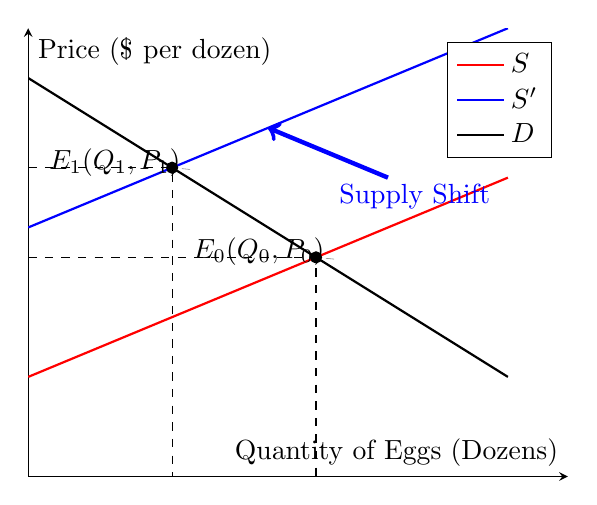
\begin{tikzpicture}
  \begin{axis}[
    axis lines=middle,
    xlabel={Quantity of Eggs (Dozens)},
    ylabel={Price (\$ per dozen)},
    xtick=\empty, ytick=\empty,
    xmin=0, xmax=9, ymin=0, ymax=9, % Adjusted limits for better visibility
    legend pos= north east,
    legend cell align={left} % Align legend text
  ]
  \addplot[name path=S,domain=0:8, color=red, thick] {0.5*x+2};
  \addlegendentry{$S$}
  \addplot[name path=S2,domain=0:8, color=blue, thick] {0.5*x+5};
  \addlegendentry{$S'$}
  \addplot[name path=D,domain=0:8, color=black, thick] {-0.75*x+8}; % Changed color for distinction
  \addlegendentry{$D$}
  
  % Equilibrium points calculation (Intersection of S and D, S' and D)
  % E0: 0.5*x + 2 = -0.75*x + 8 => 1.25*x = 6 => x = 4.8, y = 0.5*4.8 + 2 = 4.4
  % E1: 0.5*x + 5 = -0.75*x + 8 => 1.25*x = 3 => x = 2.4, y = 0.5*2.4 + 5 = 6.2
  
  \addplot[only marks, mark=*, mark size=2pt] coordinates {(4.8,4.4)} node[pin={[pin distance=-0.5cm]135:{$E_0(Q_0, P_0)$}}] {}; % Label P0, Q0
  \addplot[only marks, mark=*, mark size=2pt] coordinates {(2.4,6.2)} node[pin={[pin distance=-0.5cm]135:{$E_1(Q_1, P_1)$}}] {}; % Label P1, Q1

  % Dashed lines to axes for E0
  \draw[dashed] (axis cs:0,4.4) -- (axis cs:4.8,4.4) -- (axis cs:4.8,0);
  \node[left] at (axis cs:0,4.4) {$P_0$};
  \node[below] at (axis cs:4.8,0) {$Q_0$};
  
  % Dashed lines to axes for E1
  \draw[dashed] (axis cs:0,6.2) -- (axis cs:2.4,6.2) -- (axis cs:2.4,0);
  \node[left] at (axis cs:0,6.2) {$P_1$};
  \node[below] at (axis cs:2.4,0) {$Q_1$};

  % Arrow indicating shift
  \draw[->, blue, ultra thick] (axis cs:6,6) -- (axis cs:4,7) node[midway, below right, yshift=-0.25cm] {Supply Shift};

  \end{axis}
\end{tikzpicture}
\caption{Supply and demand shifts in the egg market due to bird flu.}
\label{fig:egg_market}
\end{figure}

This shock heavily impacted related businesses like Daquan's RVA Cafe, which uses thousands of eggs weekly. Increased egg costs function as a leftward shift in the café's supply curve for egg dishes (from $S_{\text{caf\'{e}}}$ to $S'_{\text{caf\'{e}}}$ in Figure 2). To maintain profitability, cafés like Daquan's had to raise menu prices, sometimes adding explicit surcharges—he added about \$1 to egg dishes. The price hike depended on factors like the dish's reliance on eggs (omelets vs. pancakes), customer price sensitivity, and the availability of substitutes, which Daquan noted are hard to find for core breakfast items.

\begin{figure}[H]
\centering
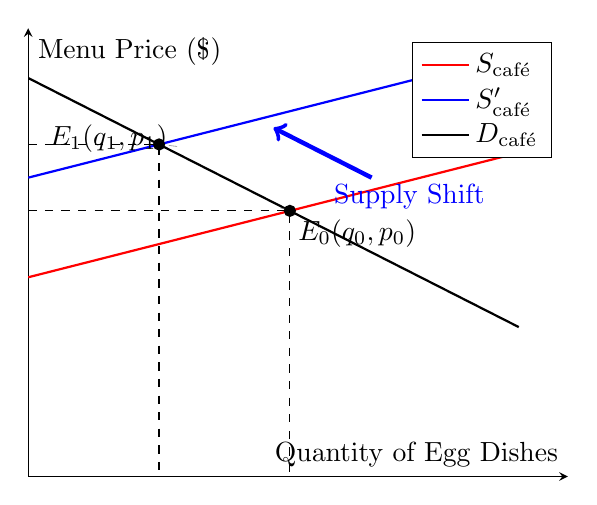
\begin{tikzpicture}
  \begin{axis}[
    axis lines=middle,
    xlabel={Quantity of Egg Dishes},
    ylabel={Menu Price (\$)},
    xtick=\empty, ytick=\empty,
    xmin=0, xmax=11, ymin=0, ymax=9, % Adjusted limits
    legend pos= north east,
    legend cell align={left}
  ]
  \addplot[name path=Sc,domain=0:10, color=red, thick] {0.25*x+4};
  \addlegendentry{$S_{\text{caf\'{e}}}$}
  \addplot[name path=Sc2,domain=0:10, color=blue, thick] {0.25*x+6};
  \addlegendentry{$S'_{\text{caf\'{e}}}$}
  \addplot[name path=Dc,domain=0:10, color=black, thick] {-0.5*x+8};
  \addlegendentry{$D_{\text{caf\'{e}}}$}
  
  % Equilibrium points calculation
  % E0: 0.25*x + 4 = -0.5*x + 8 => 0.75*x = 4 => x = 5.3333, y = 0.25*5.3333 + 4 = 5.3333
  % E1: 0.25*x + 6 = -0.5*x + 8 => 0.75*x = 2 => x = 2.6667, y = 0.25*2.6667 + 6 = 6.6667

  \addplot[only marks, mark=*, mark size=2pt] coordinates {(5.3333,5.3333)} node[pin={[pin distance=-0.2cm]315:{$E_0(q_0, p_0)$}}] {}; % Label p0, q0
  \addplot[only marks, mark=*, mark size=2pt] coordinates {(2.6667,6.667)} node[pin={[pin distance=-0.5cm]135:{$E_1(q_1, p_1)$}}] {}; % Label p1, q1

  % Dashed lines to axes for E0
  \draw[dashed] (axis cs:0,5.3333) -- (axis cs:5.3333,5.3333) -- (axis cs:5.3333,0);
   \node[left] at (axis cs:0,5.3333) {$p_0$};
   \node[below] at (axis cs:5.3333,0) {$q_0$};
   
  % Dashed lines to axes for E1
  \draw[dashed] (axis cs:0,6.6667) -- (axis cs:2.6667,6.6667) -- (axis cs:2.6667,0);
   \node[left] at (axis cs:0,6.6667) {$p_1$};
   \node[below] at (axis cs:2.6667,0) {$q_1$};

  % Arrow indicating shift
  \draw[->, blue, ultra thick] (axis cs:7,6) -- (axis cs:5,7) node[midway, below right, yshift = -0.25cm] {Supply Shift};

  \end{axis}
\end{tikzpicture}
\caption{Supply shift in the breakfast caf\'{e} market due to higher egg costs.}
\label{fig:cafe_market}
\end{figure}

The bird flu scenario also reveals externalities related to potential solutions like vaccination. Vaccinating the nation's 300 million hens offers a private benefit (farmer's flock protected) and a crucial social benefit (reduced disease spread, stable supply/prices). This latter benefit is a \emph{positive externality}; individual farmers don't capture the full societal value of preventing large outbreaks. Therefore, market forces alone may lead to under-vaccination. Significant hurdles exist, including the logistical nightmare of vaccinating so many birds and fears among broiler chicken producers about losing export markets if trading partners reject vaccinated poultry due to concerns about masked infections. Despite these issues, the egg industry increasingly favors vaccination. A government subsidy could help bridge the gap between private costs and social benefits, promoting vaccination levels closer to the social optimum and enhancing overall welfare.

Tracing these effects—from the supply shock impacting farmers to consumer and café price adjustments to the complexities of vaccination—demonstrates the power of supply and demand principles in explaining how seemingly distant events influence everyday economic life.

\end{doublespace}
\end{document}